% Options for packages loaded elsewhere
\PassOptionsToPackage{unicode}{hyperref}
\PassOptionsToPackage{hyphens}{url}
\PassOptionsToPackage{dvipsnames,svgnames,x11names}{xcolor}
%
\documentclass[
  letterpaper,
  DIV=11,
  numbers=noendperiod]{scrreprt}

\usepackage{amsmath,amssymb}
\usepackage{iftex}
\ifPDFTeX
  \usepackage[T1]{fontenc}
  \usepackage[utf8]{inputenc}
  \usepackage{textcomp} % provide euro and other symbols
\else % if luatex or xetex
  \usepackage{unicode-math}
  \defaultfontfeatures{Scale=MatchLowercase}
  \defaultfontfeatures[\rmfamily]{Ligatures=TeX,Scale=1}
\fi
\usepackage{lmodern}
\ifPDFTeX\else  
    % xetex/luatex font selection
\fi
% Use upquote if available, for straight quotes in verbatim environments
\IfFileExists{upquote.sty}{\usepackage{upquote}}{}
\IfFileExists{microtype.sty}{% use microtype if available
  \usepackage[]{microtype}
  \UseMicrotypeSet[protrusion]{basicmath} % disable protrusion for tt fonts
}{}
\makeatletter
\@ifundefined{KOMAClassName}{% if non-KOMA class
  \IfFileExists{parskip.sty}{%
    \usepackage{parskip}
  }{% else
    \setlength{\parindent}{0pt}
    \setlength{\parskip}{6pt plus 2pt minus 1pt}}
}{% if KOMA class
  \KOMAoptions{parskip=half}}
\makeatother
\usepackage{xcolor}
\setlength{\emergencystretch}{3em} % prevent overfull lines
\setcounter{secnumdepth}{5}
% Make \paragraph and \subparagraph free-standing
\makeatletter
\ifx\paragraph\undefined\else
  \let\oldparagraph\paragraph
  \renewcommand{\paragraph}{
    \@ifstar
      \xxxParagraphStar
      \xxxParagraphNoStar
  }
  \newcommand{\xxxParagraphStar}[1]{\oldparagraph*{#1}\mbox{}}
  \newcommand{\xxxParagraphNoStar}[1]{\oldparagraph{#1}\mbox{}}
\fi
\ifx\subparagraph\undefined\else
  \let\oldsubparagraph\subparagraph
  \renewcommand{\subparagraph}{
    \@ifstar
      \xxxSubParagraphStar
      \xxxSubParagraphNoStar
  }
  \newcommand{\xxxSubParagraphStar}[1]{\oldsubparagraph*{#1}\mbox{}}
  \newcommand{\xxxSubParagraphNoStar}[1]{\oldsubparagraph{#1}\mbox{}}
\fi
\makeatother


\providecommand{\tightlist}{%
  \setlength{\itemsep}{0pt}\setlength{\parskip}{0pt}}\usepackage{longtable,booktabs,array}
\usepackage{calc} % for calculating minipage widths
% Correct order of tables after \paragraph or \subparagraph
\usepackage{etoolbox}
\makeatletter
\patchcmd\longtable{\par}{\if@noskipsec\mbox{}\fi\par}{}{}
\makeatother
% Allow footnotes in longtable head/foot
\IfFileExists{footnotehyper.sty}{\usepackage{footnotehyper}}{\usepackage{footnote}}
\makesavenoteenv{longtable}
\usepackage{graphicx}
\makeatletter
\def\maxwidth{\ifdim\Gin@nat@width>\linewidth\linewidth\else\Gin@nat@width\fi}
\def\maxheight{\ifdim\Gin@nat@height>\textheight\textheight\else\Gin@nat@height\fi}
\makeatother
% Scale images if necessary, so that they will not overflow the page
% margins by default, and it is still possible to overwrite the defaults
% using explicit options in \includegraphics[width, height, ...]{}
\setkeys{Gin}{width=\maxwidth,height=\maxheight,keepaspectratio}
% Set default figure placement to htbp
\makeatletter
\def\fps@figure{htbp}
\makeatother
% definitions for citeproc citations
\NewDocumentCommand\citeproctext{}{}
\NewDocumentCommand\citeproc{mm}{%
  \begingroup\def\citeproctext{#2}\cite{#1}\endgroup}
\makeatletter
 % allow citations to break across lines
 \let\@cite@ofmt\@firstofone
 % avoid brackets around text for \cite:
 \def\@biblabel#1{}
 \def\@cite#1#2{{#1\if@tempswa , #2\fi}}
\makeatother
\newlength{\cslhangindent}
\setlength{\cslhangindent}{1.5em}
\newlength{\csllabelwidth}
\setlength{\csllabelwidth}{3em}
\newenvironment{CSLReferences}[2] % #1 hanging-indent, #2 entry-spacing
 {\begin{list}{}{%
  \setlength{\itemindent}{0pt}
  \setlength{\leftmargin}{0pt}
  \setlength{\parsep}{0pt}
  % turn on hanging indent if param 1 is 1
  \ifodd #1
   \setlength{\leftmargin}{\cslhangindent}
   \setlength{\itemindent}{-1\cslhangindent}
  \fi
  % set entry spacing
  \setlength{\itemsep}{#2\baselineskip}}}
 {\end{list}}
\usepackage{calc}
\newcommand{\CSLBlock}[1]{\hfill\break\parbox[t]{\linewidth}{\strut\ignorespaces#1\strut}}
\newcommand{\CSLLeftMargin}[1]{\parbox[t]{\csllabelwidth}{\strut#1\strut}}
\newcommand{\CSLRightInline}[1]{\parbox[t]{\linewidth - \csllabelwidth}{\strut#1\strut}}
\newcommand{\CSLIndent}[1]{\hspace{\cslhangindent}#1}

\KOMAoption{captions}{tableheading}
\makeatletter
\@ifpackageloaded{bookmark}{}{\usepackage{bookmark}}
\makeatother
\makeatletter
\@ifpackageloaded{caption}{}{\usepackage{caption}}
\AtBeginDocument{%
\ifdefined\contentsname
  \renewcommand*\contentsname{Table of contents}
\else
  \newcommand\contentsname{Table of contents}
\fi
\ifdefined\listfigurename
  \renewcommand*\listfigurename{List of Figures}
\else
  \newcommand\listfigurename{List of Figures}
\fi
\ifdefined\listtablename
  \renewcommand*\listtablename{List of Tables}
\else
  \newcommand\listtablename{List of Tables}
\fi
\ifdefined\figurename
  \renewcommand*\figurename{Figure}
\else
  \newcommand\figurename{Figure}
\fi
\ifdefined\tablename
  \renewcommand*\tablename{Table}
\else
  \newcommand\tablename{Table}
\fi
}
\@ifpackageloaded{float}{}{\usepackage{float}}
\floatstyle{ruled}
\@ifundefined{c@chapter}{\newfloat{codelisting}{h}{lop}}{\newfloat{codelisting}{h}{lop}[chapter]}
\floatname{codelisting}{Listing}
\newcommand*\listoflistings{\listof{codelisting}{List of Listings}}
\makeatother
\makeatletter
\makeatother
\makeatletter
\@ifpackageloaded{caption}{}{\usepackage{caption}}
\@ifpackageloaded{subcaption}{}{\usepackage{subcaption}}
\makeatother

\ifLuaTeX
  \usepackage{selnolig}  % disable illegal ligatures
\fi
\usepackage{bookmark}

\IfFileExists{xurl.sty}{\usepackage{xurl}}{} % add URL line breaks if available
\urlstyle{same} % disable monospaced font for URLs
\hypersetup{
  pdftitle={SOCA-D554 - Mobilisations, genre et identités professionnelles - 2024- 25},
  pdfauthor={Pierre Brasseur},
  colorlinks=true,
  linkcolor={blue},
  filecolor={Maroon},
  citecolor={Blue},
  urlcolor={Blue},
  pdfcreator={LaTeX via pandoc}}


\title{SOCA-D554 - Mobilisations, genre et identités professionnelles -
2024- 25}
\author{Pierre Brasseur}
\date{2025-02-07}

\begin{document}
\maketitle

\renewcommand*\contentsname{Table of contents}
{
\hypersetup{linkcolor=}
\setcounter{tocdepth}{2}
\tableofcontents
}

\bookmarksetup{startatroot}

\chapter*{Présentation du cours}\label{pruxe9sentation-du-cours}
\addcontentsline{toc}{chapter}{Présentation du cours}

\markboth{Présentation du cours}{Présentation du cours}

\bookmarksetup{startatroot}

\chapter*{}\label{section}
\addcontentsline{toc}{chapter}{}

\markboth{}{}

\bookmarksetup{startatroot}

\chapter{Introduction}\label{introduction}

Commencer par un exercice de déconstruction des évidences :

Faire lister aux étudiants ce qui relève selon eux du ``naturel'' et du
``culturel'' Analyser collectivement ces catégorisations

\section{Ressources bibliographiques
essentielles}\label{ressources-bibliographiques-essentielles}

\begin{itemize}
\tightlist
\item
  Delphy, Christine (2001) ``L'ennemi principal. Penser le genre'' -
  Fondamental pour la section sur l'approche française
\item
  Dorlin, Elsa (2008) ``Sexe, genre et sexualités'' - Excellente
  synthèse historique
\item
  Fausto-Sterling, Anne (2012) ``Corps en tous genres'' - Pour la partie
  médicale
\item
  Bereni et al.~(2020) ``Introduction aux études sur le genre'' - Manuel
  de référence actualisé
\end{itemize}

Séance 1 - Définir le genre et le travail Pierre Brasseur, 2024
Objectifs du cours

Définir et articuler les notions de sexe, genre et sexualité à travers
leur construction historique et sociale Explorer la généalogie de ces
concepts en France et dans les pays anglo-saxons Analyser la circulation
de ces notions entre différents champs (médical, féministe, académique)
Développer une approche critique des catégorisations naturalisées

\bookmarksetup{startatroot}

\chapter{Exercice d'ouverture : Déconstruire les évidences sur le
genre}\label{exercice-douverture-duxe9construire-les-uxe9vidences-sur-le-genre}

\section{Objectif pédagogique}\label{objectif-puxe9dagogique}

Faire émerger et questionner les représentations spontanées des
étudiant·es sur ce qui relève du ``naturel'' et du ``culturel'' dans les
différences hommes/femmes.

\section{Déroulé de l'exercice (30
minutes)}\label{duxe9rouluxe9-de-lexercice-30-minutes}

\subsection{Phase 1 : Travail individuel (5
minutes)}\label{phase-1-travail-individuel-5-minutes}

\begin{itemize}
\tightlist
\item
  Distribuer une feuille avec deux colonnes : ``Naturel'' et
  ``Culturel''
\item
  Consigne : ``Listez les différences entre hommes et femmes que vous
  considérez comme naturelles ou culturelles''
\item
  Encourager les étudiant·es à noter tout ce qui leur vient à l'esprit
\end{itemize}

\subsection{Phase 2 : Mise en commun (10
minutes)}\label{phase-2-mise-en-commun-10-minutes}

\begin{itemize}
\tightlist
\item
  Au tableau, créer deux colonnes identiques
\item
  Noter les propositions des étudiant·es en préservant leurs
  catégorisations
\item
  Favoriser la participation de tous·tes
\item
  Ne pas commenter les propositions à ce stade
\end{itemize}

\subsection{Phase 3 : Discussion critique (15
minutes)}\label{phase-3-discussion-critique-15-minutes}

Questionner collectivement les catégorisations à travers plusieurs axes
:

\begin{enumerate}
\def\labelenumi{\arabic{enumi}.}
\tightlist
\item
  \textbf{Historicité des catégories}

  \begin{itemize}
  \tightlist
  \item
    ``Ces différences ont-elles toujours existé ?''
  \item
    ``Sont-elles les mêmes dans toutes les sociétés ?''
  \end{itemize}
\item
  \textbf{Construction du naturel}

  \begin{itemize}
  \tightlist
  \item
    ``Comment savons-nous que telle différence est naturelle ?''
  \item
    ``Quelles sont nos sources de connaissance ?''
  \end{itemize}
\item
  \textbf{Variations culturelles}

  \begin{itemize}
  \tightlist
  \item
    ``Ces différences sont-elles universelles ?''
  \item
    ``Connaissez-vous des contre-exemples ?''
  \end{itemize}
\end{enumerate}

\section{Exemples de catégorisations fréquentes à
déconstruire}\label{exemples-de-catuxe9gorisations-fruxe9quentes-uxe0-duxe9construire}

\textbf{Souvent classé comme ``naturel''} : - Force physique - Maternité
- Hormones - Voix - Morphologie

\textbf{Souvent classé comme ``culturel''} : - Vêtements - Métiers -
Comportements - Rôles sociaux - Goûts

\section{Points théoriques à
introduire}\label{points-thuxe9oriques-uxe0-introduire}

\begin{enumerate}
\def\labelenumi{\arabic{enumi}.}
\tightlist
\item
  La naturalisation comme processus social
\item
  Le rôle des sciences dans la construction des différences
\item
  L'historicité des catégories de sexe et de genre
\item
  L'imbrication du biologique et du social
\end{enumerate}

\bookmarksetup{startatroot}

\chapter{}\label{section-1}

Je vais vous proposer une version enrichie de cette partie qui intègre à
la fois les aspects historiques et une approche pédagogique structurée.

\bookmarksetup{startatroot}

\chapter{Généalogie médicale du genre (45
min)}\label{guxe9nuxe9alogie-muxe9dicale-du-genre-45-min}

La rupture épistémologique du XVIIIe siècle (20 min) Introduction (5
min) Accroche pédagogique Commencer par montrer deux représentations
anatomiques aux étudiants :

Une planche de Vésale (XVIe siècle) montrant les organes génitaux comme
analogues Une planche du XIXe siècle insistant sur les différences
anatomiques

Questions d'ouverture aux étudiants

``Que remarquez-vous comme différences entre ces deux représentations
?'' ``Comment expliquez-vous ce changement de perspective ?'' ``Quelles
conceptions de la différence des sexes reflètent-elles ?''

Présentation du cadre théorique Objectifs du cours :

Comprendre la transformation radicale dans la conception médicale des
sexes Analyser les implications sociales et politiques de ce changement
Réfléchir sur les liens entre savoir médical et société

Concepts clés à définir :

\begin{description}
\tightlist
\item[Épistémologie : étude de la construction des savoirs Dimorphisme
sexuel]
conception de deux sexes biologiquement distincts Naturalisation :
processus par lequel des différences sociales sont présentées comme
naturelles
\end{description}

\bookmarksetup{startatroot}

\chapter{}\label{section-2}

\bookmarksetup{startatroot}

\chapter{Le modèle du sexe unique
(Antiquité-XVIIIe)}\label{le-moduxe8le-du-sexe-unique-antiquituxe9-xviiie}

\section{1. Les fondements antiques (10
min)}\label{les-fondements-antiques-10-min}

\subsection{Théorie galénique}\label{thuxe9orie-galuxe9nique}

\begin{itemize}
\tightlist
\item
  Corps pensé comme un continuum de perfection

  \begin{itemize}
  \tightlist
  \item
    Le masculin : forme la plus aboutie
  \item
    Le féminin : version imparfaite
  \end{itemize}
\end{itemize}

\subsubsection{La perfection comme
chaleur}\label{la-perfection-comme-chaleur}

Dans le système galénique, la différence entre les sexes n'est pas une
différence de nature mais de degré. Le corps masculin est considéré
comme ayant atteint un degré supérieur de perfection grâce à un niveau
de chaleur plus élevé. Cette chaleur permet le développement complet des
organes vers l'extérieur.

\subsubsection{Le défaut de chaleur
féminin}\label{le-duxe9faut-de-chaleur-fuxe9minin}

Le corps féminin est théorisé comme manquant de la chaleur nécessaire
pour extérioriser pleinement ses organes. C'est ce ``défaut'' qui
explique l'inversion et l'intériorisation des organes génitaux. Les
organes féminins sont donc les mêmes que les organes masculins, mais
restés à l'intérieur par manque de chaleur.

\subsection{Théorie des humeurs et
tempéraments}\label{thuxe9orie-des-humeurs-et-tempuxe9raments}

\begin{itemize}
\tightlist
\item
  Le système humoral galénique définit les différences entre les sexes
  selon quatre qualités fondamentales :

  \begin{itemize}
  \tightlist
  \item
    Chaud vs Froid
  \item
    Sec vs Humide
  \end{itemize}
\end{itemize}

\subsubsection{Impact sur la formation des
organes}\label{impact-sur-la-formation-des-organes}

\begin{itemize}
\tightlist
\item
  La chaleur est considérée comme la force qui permet :

  \begin{itemize}
  \tightlist
  \item
    La coagulation du sang menstruel en semence
  \item
    L'extériorisation des organes reproducteurs
  \item
    Le développement des caractères masculins
  \end{itemize}
\end{itemize}

\subsubsection{Applications pratiques}\label{applications-pratiques}

Cette théorie avait des implications concrètes en médecine : - Régimes
alimentaires différenciés selon le sexe - Traitements visant à
``rééquilibrer'' les humeurs - Conseils d'hygiène de vie genrés

Cette conception unifiée du corps humain, basée sur un continuum plutôt
qu'une opposition binaire, va persister jusqu'au XVIIIe siècle. Elle
structure profondément la pensée médicale et influence directement les
pratiques thérapeutiques.

\bookmarksetup{startatroot}

\chapter{2. Héritage médiéval et Renaissance (10
min)}\label{huxe9ritage-muxe9diuxe9val-et-renaissance-10-min}

\section{La transmission du savoir
antique}\label{la-transmission-du-savoir-antique}

\subsection{A. Le rôle clé des traductions arabes (XIe-XIIe
siècles)}\label{a.-le-ruxf4le-cluxe9-des-traductions-arabes-xie-xiie-siuxe8cles}

\begin{itemize}
\tightlist
\item
  Centre de traduction de Tolède comme plaque tournante :

  \begin{itemize}
  \tightlist
  \item
    Traduction de Galien via l'arabe vers le latin
  \item
    Synthèse des commentaires arabes (Avicenne, Rhazès)
  \item
    Enrichissement du corpus par les observations arabes
  \end{itemize}
\end{itemize}

\subsection{B. La circulation des manuscrits
médicaux}\label{b.-la-circulation-des-manuscrits-muxe9dicaux}

\begin{itemize}
\tightlist
\item
  \textbf{Principaux traités} :

  \begin{itemize}
  \tightlist
  \item
    ``Canon'' d'Avicenne (référence médicale jusqu'au XVIIe)
  \item
    ``De usu partium'' de Galien
  \item
    Compilations médiévales (Salernitains)
  \end{itemize}
\item
  \textbf{Centres de diffusion} :

  \begin{itemize}
  \tightlist
  \item
    Écoles de médecine (Salerne, Montpellier)
  \item
    Monastères comme lieux de copie
  \item
    Universités naissantes
  \end{itemize}
\end{itemize}

\subsection{C. Persistance et adaptation du modèle
unisexe}\label{c.-persistance-et-adaptation-du-moduxe8le-unisexe}

\begin{enumerate}
\def\labelenumi{\arabic{enumi}.}
\tightlist
\item
  \textbf{Continuité conceptuelle} :

  \begin{itemize}
  \tightlist
  \item
    Maintien de la théorie des humeurs
  \item
    Vision hiérarchique des corps
  \item
    Analogie structurelle des organes
  \end{itemize}
\item
  \textbf{Intégration aux savoirs chrétiens} :

  \begin{itemize}
  \tightlist
  \item
    Adaptation à la théologie (création d'Adam et Ève)
  \item
    Réinterprétation de la différence des sexes
  \item
    Maintien d'une hiérarchie naturelle
  \end{itemize}
\item
  \textbf{Innovation dans les pratiques} :

  \begin{itemize}
  \tightlist
  \item
    Développement des dissections universitaires
  \item
    Premières illustrations anatomiques détaillées
  \item
    Début d'observations systématiques
  \end{itemize}
\end{enumerate}

\subsection{D. Les tensions
émergentes}\label{d.-les-tensions-uxe9mergentes}

\begin{itemize}
\tightlist
\item
  Contradiction entre observations anatomiques et théorie
\item
  Questions sur la génération et le rôle des sexes
\item
  Débuts d'une remise en question du modèle unique
\end{itemize}

Cette période de transmission montre : - La remarquable stabilité du
modèle unisexe - Son adaptation à différents contextes culturels -
L'émergence progressive de ses limites

\subsection{}\label{section-3}

\bookmarksetup{startatroot}

\chapter{Développement de l'anatomie (XIVe-XVIe
siècles)}\label{duxe9veloppement-de-lanatomie-xive-xvie-siuxe8cles}

\section{1. Les dissections publiques (à partir du
XIVe)}\label{les-dissections-publiques-uxe0-partir-du-xive}

\subsection{La pratique de la
dissection}\label{la-pratique-de-la-dissection}

\begin{itemize}
\tightlist
\item
  Cadre institutionnel :

  \begin{itemize}
  \tightlist
  \item
    Autorisations papales et universitaires
  \item
    Amphithéâtres d'anatomie
  \item
    Calendrier ritualisé (hiver)
  \end{itemize}
\end{itemize}

\subsection{Organisation des séances}\label{organisation-des-suxe9ances}

\begin{itemize}
\tightlist
\item
  Hiérarchie des rôles :

  \begin{itemize}
  \tightlist
  \item
    Le professeur qui lit (lector)
  \item
    Le chirurgien qui dissèque (sector)
  \item
    Les étudiants qui observent
  \end{itemize}
\item
  Ordre établi de la dissection :

  \begin{itemize}
  \tightlist
  \item
    Des organes périssables aux plus stables
  \item
    Des structures externes aux internes
  \end{itemize}
\end{itemize}

\section{2. Les planches anatomiques}\label{les-planches-anatomiques}

\subsection{Evolution des
représentations}\label{evolution-des-repruxe9sentations}

\begin{itemize}
\tightlist
\item
  \textbf{Avant 1500} :

  \begin{itemize}
  \tightlist
  \item
    Schémas simplifiés
  \item
    Forte influence des textes antiques
  \item
    Peu d'observations directes
  \end{itemize}
\item
  \textbf{Après 1500} :

  \begin{itemize}
  \tightlist
  \item
    Vésale (1543) : révolution visuelle
  \item
    Précision croissante des détails
  \item
    Maintien du cadre galénique dans l'interprétation
  \end{itemize}
\end{itemize}

\section{3. La terminologie
anatomique}\label{la-terminologie-anatomique}

\subsection{Vocabulaire des
correspondances}\label{vocabulaire-des-correspondances}

\begin{itemize}
\tightlist
\item
  \textbf{Exemples d'analogies} :

  \begin{itemize}
  \tightlist
  \item
    ``Orchis'' pour ovaires et testicules
  \item
    ``Vases spermatiques'' pour tous les conduits
  \item
    ``Col'' pour désigner vagin et pénis
  \end{itemize}
\end{itemize}

\subsection{Logique descriptive}\label{logique-descriptive}

\begin{itemize}
\tightlist
\item
  \textbf{Principe d'homologie} :

  \begin{itemize}
  \tightlist
  \item
    Structures ``tournées vers l'intérieur/extérieur''
  \item
    Description par comparaison
  \item
    Variations de position plus que de nature
  \end{itemize}
\end{itemize}

Cette période montre : - L'importance croissante de l'observation
directe - La persistance du cadre interprétatif ancien - Les tensions
entre voir et savoir

Cet enseignement peut être enrichi par : - L'analyse de planches
anatomiques d'époque - La lecture d'extraits de traités anatomiques -
L'étude de la terminologie médicale actuelle et ses origines

\section{}\label{section-4}

\bookmarksetup{startatroot}

\chapter{3. Implications conceptuelles (10
min)}\label{implications-conceptuelles-10-min}

\section{Vision hiérarchique des
corps}\label{vision-hiuxe9rarchique-des-corps}

\subsection{A. L'échelle de perfection
corporelle}\label{a.-luxe9chelle-de-perfection-corporelle}

\subsubsection{Fondements théoriques}\label{fondements-thuxe9oriques}

\begin{itemize}
\tightlist
\item
  Conception verticale du vivant :

  \begin{itemize}
  \tightlist
  \item
    Sommet : homme adulte parfait
  \item
    Échelons intermédiaires : femmes, enfants
  \item
    Base : êtres imparfaits
  \end{itemize}
\end{itemize}

\subsubsection{Critères de perfection}\label{crituxe8res-de-perfection}

\begin{itemize}
\tightlist
\item
  La chaleur comme marqueur principal :

  \begin{itemize}
  \tightlist
  \item
    Maximum : corps masculin adulte
  \item
    Déficit : corps féminin, corps juvénile
  \end{itemize}
\item
  Autres indicateurs :

  \begin{itemize}
  \tightlist
  \item
    Équilibre des humeurs
  \item
    Développement des organes
  \item
    Force physique et morale
  \end{itemize}
\end{itemize}

\subsection{B. La possibilité théorique de
transformation}\label{b.-la-possibilituxe9-thuxe9orique-de-transformation}

\subsubsection{Mobilité sur
l'échelle}\label{mobilituxe9-sur-luxe9chelle}

\begin{itemize}
\tightlist
\item
  Transformations possibles dans les deux sens :

  \begin{itemize}
  \tightlist
  \item
    Ascendantes (vers le masculin)
  \item
    Descendantes (vers le féminin)
  \end{itemize}
\end{itemize}

\subsubsection{Facteurs de
transformation}\label{facteurs-de-transformation}

\begin{itemize}
\tightlist
\item
  Influences environnementales :

  \begin{itemize}
  \tightlist
  \item
    Régime alimentaire
  \item
    Mode de vie
  \item
    Climat
  \end{itemize}
\item
  États physiologiques :

  \begin{itemize}
  \tightlist
  \item
    Âge
  \item
    Maladie
  \item
    Exercice
  \end{itemize}
\end{itemize}

\subsection{C. La peur de la
``régression''}\label{c.-la-peur-de-la-ruxe9gression}

\subsubsection{Anxiétés sociales et
médicales}\label{anxiuxe9tuxe9s-sociales-et-muxe9dicales}

\begin{itemize}
\tightlist
\item
  Craintes de la ``féminisation'' :

  \begin{itemize}
  \tightlist
  \item
    Perte de chaleur vitale
  \item
    Affaiblissement moral
  \item
    Déchéance sociale
  \end{itemize}
\end{itemize}

\subsubsection{Manifestations pratiques}\label{manifestations-pratiques}

\begin{itemize}
\tightlist
\item
  Prescriptions médicales :

  \begin{itemize}
  \tightlist
  \item
    Régimes ``fortifiants''
  \item
    Exercices ``virils''
  \item
    Évitement des ``excès''
  \end{itemize}
\end{itemize}

\subsection{Implications
contemporaines}\label{implications-contemporaines}

\begin{itemize}
\tightlist
\item
  Persistances de ces conceptions :

  \begin{itemize}
  \tightlist
  \item
    Dans le langage médical
  \item
    Dans certaines pratiques
  \item
    Dans les représentations populaires
  \end{itemize}
\end{itemize}

Cette vision hiérarchique révèle : - La dimension sociale de la pensée
médicale - Les enjeux politiques du savoir anatomique - La construction
historique des catégories de genre

\bookmarksetup{startatroot}

\chapter{Impact social et culturel du modèle
unisexe}\label{impact-social-et-culturel-du-moduxe8le-unisexe}

\section{1. Justification de l'ordre
social}\label{justification-de-lordre-social}

\subsection{Naturalisation des
hiérarchies}\label{naturalisation-des-hiuxe9rarchies}

\begin{itemize}
\tightlist
\item
  Correspondance entre ordre corporel et ordre social :

  \begin{itemize}
  \tightlist
  \item
    Perfection masculine justifiant la domination masculine
  \item
    ``Imperfection'' féminine légitimant la subordination
  \end{itemize}
\item
  Circulation entre discours médical et politique
\end{itemize}

\subsection{Implications religieuses et
juridiques}\label{implications-religieuses-et-juridiques}

\begin{itemize}
\tightlist
\item
  Renforcement des interprétations bibliques
\item
  Fondement des droits et devoirs selon le sexe
\item
  Régulation des comportements sociaux
\end{itemize}

\section{2. Conception des rôles
genrés}\label{conception-des-ruxf4les-genruxe9s}

\subsection{Construction des identités
sociales}\label{construction-des-identituxe9s-sociales}

\begin{itemize}
\tightlist
\item
  Définition médicale des aptitudes :

  \begin{itemize}
  \tightlist
  \item
    Force et rationalité masculines
  \item
    Faiblesse et émotivité féminines
  \end{itemize}
\item
  Impact sur l'éducation et les rôles sociaux
\end{itemize}

\subsection{Normes comportementales}\label{normes-comportementales}

\begin{itemize}
\tightlist
\item
  Prescriptions différenciées :

  \begin{itemize}
  \tightlist
  \item
    Activités recommandées/interdites
  \item
    Modes de vie appropriés
  \item
    Espaces sociaux accessibles
  \end{itemize}
\end{itemize}

\section{3. Pratiques médicales et
thérapeutiques}\label{pratiques-muxe9dicales-et-thuxe9rapeutiques}

\subsection{Traitements
différenciés}\label{traitements-diffuxe9renciuxe9s}

\begin{itemize}
\tightlist
\item
  Selon le tempérament attribué :

  \begin{itemize}
  \tightlist
  \item
    Remèdes ``échauffants'' pour les femmes
  \item
    Remèdes ``rafraîchissants'' pour les hommes
  \end{itemize}
\item
  Approches préventives genrées
\end{itemize}

\subsection{Spécificités des soins}\label{spuxe9cificituxe9s-des-soins}

\begin{itemize}
\tightlist
\item
  Développement de pratiques spécialisées :

  \begin{itemize}
  \tightlist
  \item
    Émergence de la gynécologie
  \item
    Traitements des ``maladies des femmes''
  \item
    Attention particulière aux organes reproducteurs
  \end{itemize}
\end{itemize}

\subsection{Héritage contemporain}\label{huxe9ritage-contemporain}

\begin{itemize}
\tightlist
\item
  Persistances dans la médecine moderne :

  \begin{itemize}
  \tightlist
  \item
    Biais de genre dans les diagnostics
  \item
    Différences de prise en charge
  \item
    Représentations médicales sexuées
  \end{itemize}
\end{itemize}

Cette analyse montre comment un modèle médical : - Structure les
rapports sociaux - Influence durablement les pratiques - Continue
d'impacter notre vision contemporaine

\begin{quote}
Le sexe, tel que nous le connaissons\ldots{} est le produit d'un moment
historique particulier'' (Laqueur)
\end{quote}

\subsection{}\label{section-5}

\bookmarksetup{startatroot}

\chapter{A. Le modèle unisexe galénique (7-8
min)}\label{a.-le-moduxe8le-unisexe-galuxe9nique-7-8-min}

\section{Introduction à la pensée galénique (2
min)}\label{introduction-uxe0-la-pensuxe9e-galuxe9nique-2-min}

``Pour visualiser comment les anciens concevaient les sexes, imaginez
retourner un gant : la même structure, mais inversée. C'est ainsi que
Galien, au IIe siècle, concevait les organes génitaux.''

\section{1. Principes fondamentaux (3
min)}\label{principes-fondamentaux-3-min}

\subsection{Le corps comme continuum}\label{le-corps-comme-continuum}

\begin{itemize}
\tightlist
\item
  La différence sexuelle vue comme degré de développement
\item
  Métaphore de la chaleur vitale :

  \begin{itemize}
  \tightlist
  \item
    Chaleur masculine permettant l'extériorisation
  \item
    ``Froid'' féminin maintenant l'intériorisation
  \end{itemize}
\item
  Un seul sexe, deux manifestations
\end{itemize}

\subsection{L'analogie structurelle}\label{lanalogie-structurelle}

\textbf{Trois correspondances fondamentales :} 1. Pénis/vagin : * Même
structure, orientation différente * ``Pénis inversé vers l'intérieur''

\begin{enumerate}
\def\labelenumi{\arabic{enumi}.}
\setcounter{enumi}{1}
\tightlist
\item
  Testicules/ovaires :

  \begin{itemize}
  \tightlist
  \item
    Mêmes organes à différentes positions
  \item
    Nommés ``orchis'' dans les deux cas
  \end{itemize}
\item
  Scrotum/utérus :

  \begin{itemize}
  \tightlist
  \item
    Poches contenant les organes reproducteurs
  \item
    Différence de localisation uniquement
  \end{itemize}
\end{enumerate}

\section{2. Sources historiques (3
min)}\label{sources-historiques-3-min}

\subsection{Analyse de documents}\label{analyse-de-documents}

\textbf{Planche de Vésale (1543)} - Projection de la planche -
Observation guidée : * Repérer les analogies * Noter la terminologie
utilisée * Identifier les correspondances

\textbf{Extrait de Galien} \textgreater{} ``La femme est plus imparfaite
que l'homme par une seule chose, qui est très importante, à savoir la
chaleur'' - Discussion du texte - Implications de cette vision

\begin{quote}
\textbf{Question pour la discussion :} ``Comment cette vision du corps
influence-t-elle encore notre façon de penser les différences sexuelles
?''
\end{quote}

\subsection{}\label{section-6}

\bookmarksetup{startatroot}

\chapter{B. La rupture du XVIIIe siècle (7-8
min)}\label{b.-la-rupture-du-xviiie-siuxe8cle-7-8-min}

\section{1. Le contexte de transformation (3
min)}\label{le-contexte-de-transformation-3-min}

\subsection{L'essor de l'anatomie
pathologique}\label{lessor-de-lanatomie-pathologique}

\begin{itemize}
\tightlist
\item
  Pratique systématique des autopsies
\item
  Développement des collections anatomiques
\item
  Nouveau regard sur les structures internes
\end{itemize}

\subsection{Innovations techniques}\label{innovations-techniques}

\begin{itemize}
\tightlist
\item
  Perfectionnement du microscope
\item
  Nouvelles techniques de conservation
\item
  Amélioration des illustrations médicales
\end{itemize}

\subsection{Contexte sociopolitique}\label{contexte-sociopolitique}

\begin{itemize}
\tightlist
\item
  Révolution française et ses idéaux
\item
  Nouvelle conception de la citoyenneté
\item
  Débats sur la place des femmes
\end{itemize}

\section{2. La révolution conceptuelle (4
min)}\label{la-ruxe9volution-conceptuelle-4-min}

\subsection{Du hiérarchique au
différentialiste}\label{du-hiuxe9rarchique-au-diffuxe9rentialiste}

\begin{itemize}
\tightlist
\item
  Abandon progressif de l'échelle de perfection
\item
  Émergence d'une pensée de la différence radicale
\item
  Opposition plutôt que continuité
\end{itemize}

\subsection{L'incommensurabilité des
sexes}\label{lincommensurabilituxe9-des-sexes}

\begin{itemize}
\tightlist
\item
  Deux natures distinctes et irréductibles
\item
  Spécificité des organes féminins
\item
  Nouvelle compréhension du corps féminin
\end{itemize}

\subsection{Révolution taxonomique}\label{ruxe9volution-taxonomique}

\begin{itemize}
\tightlist
\item
  Nouvelle nomenclature anatomique
\item
  Terminologie spécifique pour chaque sexe
\item
  Abandon des analogies traditionnelles
\end{itemize}

\section{3. Implications immédiates (1
min)}\label{implications-immuxe9diates-1-min}

\subsection{En médecine}\label{en-muxe9decine}

\begin{itemize}
\tightlist
\item
  Naissance de la gynécologie
\item
  Spécialisation des soins par sexe
\item
  Nouvelles pathologies ``féminines''
\end{itemize}

\subsection{Dans la société}\label{dans-la-sociuxe9tuxe9}

\begin{itemize}
\tightlist
\item
  Naturalisation des rôles sociaux
\item
  Séparation des sphères masculine/féminine
\item
  Nouveaux discours sur la complémentarité
\end{itemize}

\textbf{Extrait à discuter :} Pierre Roussel (1775) - \emph{Système
physique et moral de la femme} : ``La femme n'est pas seulement
différente de l'homme par ses organes, elle l'est par tout son être.''

Cette rupture épistémologique illustre comment la pensée médicale
participe à la construction sociale des catégories de sexe et de genre.

\section{}\label{section-7}

\bookmarksetup{startatroot}

\chapter{2. Implications théoriques et pratiques (15
min)}\label{implications-thuxe9oriques-et-pratiques-15-min}

\section{A. Construction du dimorphisme sexuel (8
min)}\label{a.-construction-du-dimorphisme-sexuel-8-min}

\subsection{1. Le projet scientifique du
dimorphisme}\label{le-projet-scientifique-du-dimorphisme}

\begin{itemize}
\tightlist
\item
  \textbf{Nouvelle méthode anatomique :}

  \begin{itemize}
  \tightlist
  \item
    Recherche méthodique des différences
  \item
    Documentation exhaustive des variations
  \item
    Établissement de normes sexuées
  \end{itemize}
\item
  \textbf{Révolution du langage médical :}

  \begin{itemize}
  \tightlist
  \item
    Abandon des termes analogiques
  \item
    Création d'une nomenclature spécifique
  \item
    Différenciation systématique des descriptions
  \end{itemize}
\end{itemize}

\subsection{2. L'ancrage idéologique}\label{lancrage-iduxe9ologique}

\begin{itemize}
\tightlist
\item
  \textbf{Naturalisation des inégalités :}

  \begin{itemize}
  \tightlist
  \item
    Le biologique comme destin
  \item
    Différences anatomiques justifiant les rôles sociaux
  \item
    Construction d'une ``nature féminine''
  \end{itemize}
\item
  \textbf{Théorie des tempéraments :}

  \begin{itemize}
  \tightlist
  \item
    Femme : sensibilité, fragilité, émotivité
  \item
    Homme : force, rationalité, stabilité
  \item
    Impact sur l'éducation et les droits
  \end{itemize}
\end{itemize}

\section{B. Impact sur la pratique médicale (7
min)}\label{b.-impact-sur-la-pratique-muxe9dicale-7-min}

\subsection{1. La spécialisation
médicale}\label{la-spuxe9cialisation-muxe9dicale}

\begin{itemize}
\tightlist
\item
  \textbf{Naissance de la gynécologie :}

  \begin{itemize}
  \tightlist
  \item
    Autonomisation comme spécialité
  \item
    Développement d'instruments spécifiques
  \item
    Formation de praticiens spécialisés
  \end{itemize}
\item
  \textbf{Extension du champ médical :}

  \begin{itemize}
  \tightlist
  \item
    Grossesse et accouchement
  \item
    Puberté et ménopause
  \item
    Hystérie et ``maladies des femmes''
  \end{itemize}
\end{itemize}

\subsection{2. La médicalisation
différenciée}\label{la-muxe9dicalisation-diffuxe9renciuxe9e}

\begin{itemize}
\tightlist
\item
  \textbf{Surveillance du corps féminin :}

  \begin{itemize}
  \tightlist
  \item
    Contrôle des cycles
  \item
    Régulation des comportements
  \item
    Prescriptions morales
  \end{itemize}
\item
  \textbf{Nouvelles catégories pathologiques :}

  \begin{itemize}
  \tightlist
  \item
    Troubles ``spécifiquement féminins''
  \item
    Maladies nerveuses
  \item
    Désordres de la reproduction
  \end{itemize}
\end{itemize}

\textbf{Conclusion :} Cette période établit durablement : - Une vision
binaire des corps - Une médecine genrée - Des normes biologiques et
sociales encore influentes

\textbf{Question pour la discussion :} ``Comment ces catégories
médicales historiques influencent-elles encore notre perception des
différences de genre ?''

\bookmarksetup{startatroot}

\chapter{La biologisation des différences sexuelles (XIXe-XXe
siècles)}\label{la-biologisation-des-diffuxe9rences-sexuelles-xixe-xxe-siuxe8cles}

\section{1. Anatomie pathologique et différences sexuelles
(1800-1850)}\label{anatomie-pathologique-et-diffuxe9rences-sexuelles-1800-1850}

\subsection{Nouvelle approche
anatomique}\label{nouvelle-approche-anatomique}

\begin{itemize}
\tightlist
\item
  Observation systématique des cadavres :

  \begin{itemize}
  \tightlist
  \item
    Collections anatomiques hospitalières
  \item
    Protocoles de dissection standardisés
  \item
    Relevés détaillés des particularités sexuées
  \end{itemize}
\end{itemize}

\subsection{Théorisation des
différences}\label{thuxe9orisation-des-diffuxe9rences}

\begin{itemize}
\tightlist
\item
  \textbf{Travaux fondateurs} :

  \begin{itemize}
  \tightlist
  \item
    Bichat : anatomie des tissus
  \item
    Cabanis : rapports physique/moral
  \item
    Virey : ``nature féminine''
  \end{itemize}
\item
  \textbf{Catégorisation scientifique :}

  \begin{itemize}
  \tightlist
  \item
    Système nerveux différencié
  \item
    Particularités osseuses
  \item
    Spécificités organiques
  \end{itemize}
\end{itemize}

\section{2. Émergence des nouvelles sciences du sexe
(1850-1900)}\label{uxe9mergence-des-nouvelles-sciences-du-sexe-1850-1900}

\subsection{La sexologie naissante}\label{la-sexologie-naissante}

\begin{itemize}
\tightlist
\item
  \textbf{Psychopathia Sexualis (1886)} :

  \begin{itemize}
  \tightlist
  \item
    Premier traité systématique
  \item
    Classification des comportements sexuels
  \item
    Définition des ``perversions''
  \end{itemize}
\item
  \textbf{Impact sur la compréhension du genre :}

  \begin{itemize}
  \tightlist
  \item
    Pathologisation des ``inversions''
  \item
    Normes de la masculinité/féminité
  \item
    Contrôle médical des sexualités
  \end{itemize}
\end{itemize}

\subsection{La révolution
endocrinologique}\label{la-ruxe9volution-endocrinologique}

\begin{itemize}
\tightlist
\item
  \textbf{Découvertes scientifiques :}

  \begin{itemize}
  \tightlist
  \item
    Isolement des hormones sexuelles
  \item
    Compréhension des mécanismes hormonaux
  \item
    Rôle dans le développement sexuel
  \end{itemize}
\item
  \textbf{Nouvelles perspectives thérapeutiques :}

  \begin{itemize}
  \tightlist
  \item
    Traitements hormonaux
  \item
    Interventions sur le développement
  \item
    Modification des caractères sexuels
  \end{itemize}
\end{itemize}

\section{3. Théories de la différenciation
(1900-1930)}\label{thuxe9ories-de-la-diffuxe9renciation-1900-1930}

\subsection{Bases biologiques}\label{bases-biologiques}

\begin{itemize}
\tightlist
\item
  Chromosomes sexuels
\item
  Hormones de développement
\item
  Différenciation embryonnaire
\end{itemize}

\subsection{Applications cliniques}\label{applications-cliniques}

\begin{itemize}
\tightlist
\item
  Traitement des ``anomalies''
\item
  Critères de normalité sexuelle
\item
  Protocoles thérapeutiques
\end{itemize}

Cette période établit : - Une ``science du sexe'' moderne - Des normes
biologiques strictes - Un contrôle médical accru du genre

\textbf{Document d'étude :} Extrait de Krafft-Ebing sur la
``constitution normale'' des sexes → Analyse critique en classe

\emph{Cette partie montre l'établissement des bases scientifiques
modernes de la différenciation sexuelle, tout en soulignant leurs
implications sociales et politiques.}

\subsection{Étude de cas : les protocoles de John Money
(1955)}\label{uxe9tude-de-cas-les-protocoles-de-john-money-1955}

\textbf{Contexte théorique} - Théorie de la neutralité psychosexuelle à
la naissance - Rôle déterminant de l'éducation dans l'identité de genre
- Période critique de fixation du genre (18-24 mois)

\textbf{Protocoles cliniques} - Prise en charge des enfants intersexes -
Critères de décision pour l'assignation de sexe - Importance du secret
médical - Chirurgies précoces de ``normalisation''

\textbf{Implications théoriques et pratiques} - Séparation conceptuelle
sexe/genre - Primauté accordée à l'apparence des organes génitaux -
Influence durable sur la prise en charge médicale

\subsection{}\label{section-8}

\bookmarksetup{startatroot}

\chapter{Sources historiques et études de cas pour la généalogie
médicale du
genre}\label{sources-historiques-et-uxe9tudes-de-cas-pour-la-guxe9nuxe9alogie-muxe9dicale-du-genre}

\begin{figure}[H]

{\centering 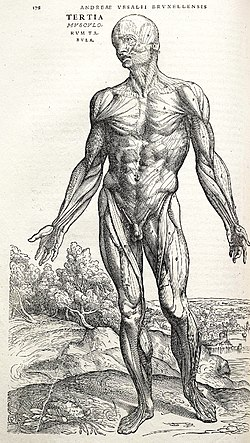
\includegraphics{images/clipboard-1755216688.png}

}

\caption{Planches anatomiques Traité d'anatomie de Vesalius (1543)
Planche des organes reproducteurs féminins/masculins montrant la théorie
du sexe unique Annotations en latin avec la terminologie de l'époque.
Source : Wikipédia}

\end{figure}%%
\begin{figure}[H]

{\centering 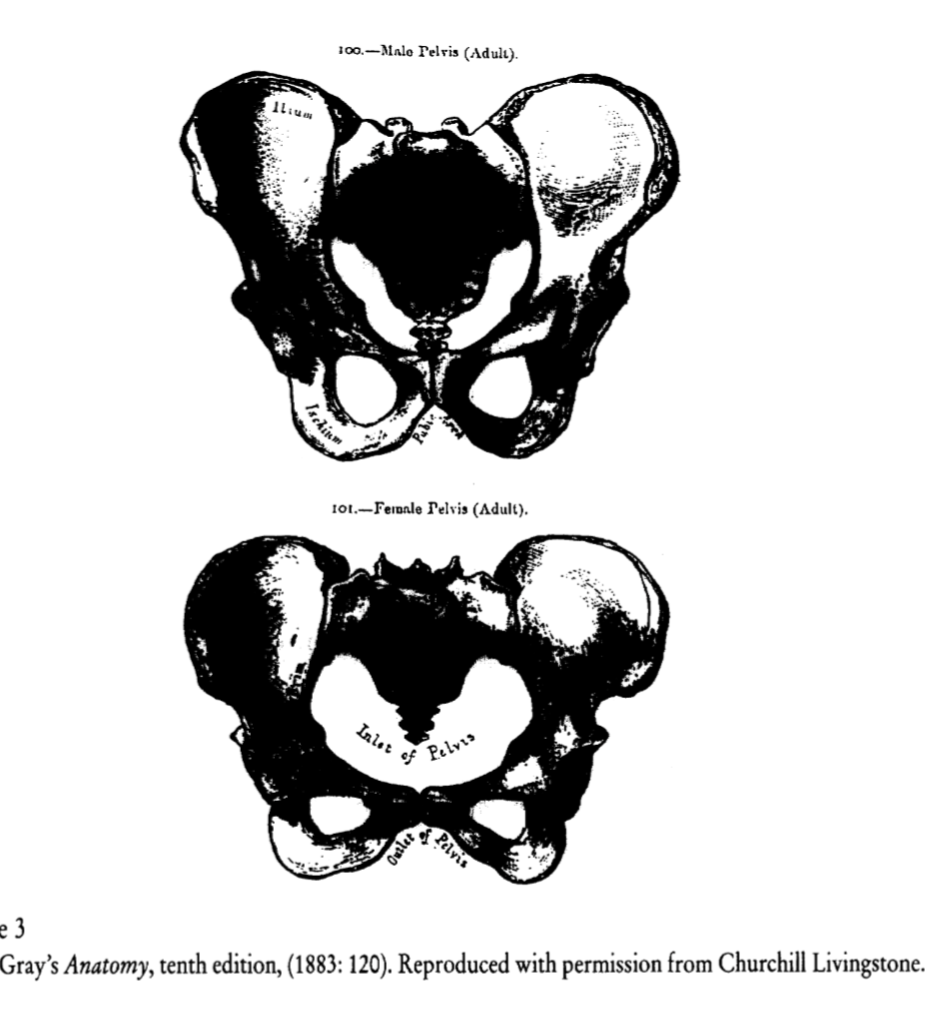
\includegraphics{images/clipboard-1285558360.png}

}

\caption{Atlas d'anatomie de Gray (1858) Représentations détaillées des
différences anatomiques homme/femme. Issu de PETERSEN, A. (1998). Sexing
the Body: Representations of Sex Differences in Gray's Anatomy, 1858 to
the Present. Body \& Society, 4(1), 1-15.}

\end{figure}%

\begin{enumerate}
\def\labelenumi{\arabic{enumi}.}
\setcounter{enumi}{2}
\tightlist
\item
  \textbf{Documents cliniques de John Money (1955)}
\end{enumerate}

\begin{itemize}
\tightlist
\item
  Schémas de protocoles d'évaluation des nouveau-nés
\item
  Grilles d'observation du comportement genré
\item
  Critères d'assignation de sexe
\end{itemize}

\section{Extraits de traités médicaux
historiques}\label{extraits-de-traituxe9s-muxe9dicaux-historiques}

\begin{enumerate}
\def\labelenumi{\arabic{enumi}.}
\tightlist
\item
  \textbf{Pierre Roussel (1775) - ``Système physique et moral de la
  femme''}
\end{enumerate}

\begin{itemize}
\tightlist
\item
  Description du ``tempérament féminin''
\item
  Justification médicale des rôles sociaux
\end{itemize}

\begin{enumerate}
\def\labelenumi{\arabic{enumi}.}
\setcounter{enumi}{1}
\tightlist
\item
  \textbf{Xavier Bichat (1801) - ``Anatomie générale''}
\end{enumerate}

\begin{itemize}
\tightlist
\item
  Théorie de la différenciation sexuelle
\item
  Descriptions des tissus et organes sexués
\end{itemize}

\begin{enumerate}
\def\labelenumi{\arabic{enumi}.}
\setcounter{enumi}{2}
\tightlist
\item
  \textbf{Cesare Lombroso (1895) - ``La femme criminelle''}
\end{enumerate}

\begin{itemize}
\tightlist
\item
  Lien entre anatomie et comportement
\item
  Théories sur les ``déviances féminines''
\end{itemize}

\section{Études de cas - Johns Hopkins
Hospital}\label{uxe9tudes-de-cas---johns-hopkins-hospital}

\subsection{Protocole de prise en charge
(1960s)}\label{protocole-de-prise-en-charge-1960s}

\begin{enumerate}
\def\labelenumi{\arabic{enumi}.}
\tightlist
\item
  Examens initiaux :

  \begin{itemize}
  \tightlist
  \item
    Critères morphologiques
  \item
    Tests hormonaux
  \item
    Examens génétiques
  \end{itemize}
\item
  Processus décisionnel :

  \begin{itemize}
  \tightlist
  \item
    Arbre de décision pour l'assignation
  \item
    Calendrier des interventions
  \item
    Protocoles de suivi
  \end{itemize}
\end{enumerate}

\subsection{Documentation
photographique}\label{documentation-photographique}

\begin{itemize}
\tightlist
\item
  Photos cliniques avant/après interventions
\item
  Radiographies et autres examens
\item
  Évolution des techniques chirurgicales
\end{itemize}

\section{Témoignages de patient·es}\label{tuxe9moignages-de-patientes}

\subsection{Archive orale (1990-2000)}\label{archive-orale-1990-2000}

\begin{itemize}
\tightlist
\item
  Récits d'expériences médicales
\item
  Impact sur la construction identitaire
\item
  Conséquences à long terme
\end{itemize}

\subsection{Documents militants intersexes
(post-2000)}\label{documents-militants-intersexes-post-2000}

\begin{itemize}
\tightlist
\item
  Critiques des protocoles médicaux
\item
  Revendications pour l'autodétermination
\item
  Évolution des pratiques médicales
\end{itemize}

\section{Utilisation pédagogique}\label{utilisation-puxe9dagogique}

\begin{enumerate}
\def\labelenumi{\arabic{enumi}.}
\tightlist
\item
  \textbf{Analyse comparative}

  \begin{itemize}
  \tightlist
  \item
    Évolution du regard médical
  \item
    Changement des critères de ``normalité''
  \item
    Transformation des pratiques
  \end{itemize}
\item
  \textbf{Discussion éthique}

  \begin{itemize}
  \tightlist
  \item
    Questions de consentement
  \item
    Rôle du secret médical
  \item
    Droits des patient·es
  \end{itemize}
\item
  \textbf{Réflexion critique}

  \begin{itemize}
  \tightlist
  \item
    Construction sociale du ``naturel''
  \item
    Pouvoir médical et normes de genre
  \item
    Résistances et changements
  \end{itemize}
\end{enumerate}

\section{Précautions d'usage}\label{pruxe9cautions-dusage}

\begin{itemize}
\tightlist
\item
  Respect de l'anonymat des patient·es
\item
  Contextualisation historique des documents
\item
  Discussion des aspects éthiques
\item
  Sensibilité aux vécus traumatiques
\end{itemize}

\section{Ressources
complémentaires}\label{ressources-compluxe9mentaires}

\begin{enumerate}
\def\labelenumi{\arabic{enumi}.}
\tightlist
\item
  \textbf{Archives médicales en ligne}

  \begin{itemize}
  \tightlist
  \item
    Wellcome Collection
  \item
    Bibliothèque numérique Medica
  \item
    Archives de la Salpêtrière
  \end{itemize}
\item
  \textbf{Fonds documentaires}

  \begin{itemize}
  \tightlist
  \item
    Archives du Planning Familial
  \item
    Collections universitaires
  \item
    Fonds d'associations intersexes
  \end{itemize}
\item
  \textbf{Témoignages contemporains}

  \begin{itemize}
  \tightlist
  \item
    Récits autobiographiques
  \item
    Documents militants
  \item
    Interviews filmées
  \end{itemize}
\end{enumerate}

\subsection{Questions pour la
discussion}\label{questions-pour-la-discussion}

\begin{enumerate}
\def\labelenumi{\arabic{enumi}.}
\tightlist
\item
  Comment la médecine a-t-elle contribué à naturaliser les différences
  de genre ?
\item
  Quel rôle ont joué les nouvelles technologies médicales dans la
  conception du sexe/genre ?
\item
  Quels sont les héritages contemporains de cette histoire médicale ?
\end{enumerate}

\subsection{Transition vers la partie
suivante}\label{transition-vers-la-partie-suivante}

Cette généalogie médicale prépare la compréhension des critiques
féministes qui vont émerger, notamment autour de la pathologisation des
corps et de la normativité médicale.

\begin{description}
\tightlist
\item[Utiliser les contradictions et questionnements émergents pour
introduire]
\begin{itemize}
\tightlist
\item[]
\item
  La nécessité d'une approche historique - L'importance de la
  construction médicale des différences - Le rôle des mouvements
  féministes dans leur critique
\end{itemize}
\end{description}

Cet exercice permet d'entrer directement dans le vif du sujet en partant
des représentations des étudiant·es, tout en introduisant la perspective
critique qui sera développée dans le cours.

Évolution historique des théories médicales (18e-19e siècles) Émergence
de la sexologie et de l'endocrinologie Étude de cas : protocoles de John
Money (1955)

1.2 Les controverses fondatrices

Le cas David Reimer et ses implications théoriques Apports critiques
d'Anne Fausto-Sterling sur la bicatégorisation

\begin{enumerate}
\def\labelenumi{\arabic{enumi}.}
\setcounter{enumi}{1}
\tightlist
\item
  Généalogies féministes (45 min) 2.1 L'émergence du concept de genre
\end{enumerate}

De Beauvoir et la dénaturalisation de la féminité Les théoriciennes
matérialistes (Delphy, Mathieu) Le genre comme rapport social de pouvoir

2.2 Les mouvements féministes et la théorisation

Le MLF et la théorisation par la lutte Contributions des féministes
matérialistes françaises Circulation internationale des concepts

\begin{enumerate}
\def\labelenumi{\arabic{enumi}.}
\setcounter{enumi}{2}
\tightlist
\item
  Le genre à la française (45 min) 3.1 Spécificités théoriques
\end{enumerate}

Les rapports sociaux de sexe vs gender L'approche matérialiste française
Le rôle du colloque de Toulouse 1982

3.2 Controverses et résistances

Débats sur la traduction de ``gender'' Tensions théoriques et politiques
Institutionnalisation des études sur le genre

\begin{enumerate}
\def\labelenumi{\arabic{enumi}.}
\setcounter{enumi}{3}
\tightlist
\item
  Vers une définition complexe du genre (45 min) 4.1 Le genre comme
  concept multidimensionnel
\end{enumerate}

Division sexuelle du travail Rapports de pouvoir Système de
représentations

4.2 Intersections et articulations

Genre et autres rapports sociaux Matérialité et symbolique Perspectives
contemporaines

Bibliographie essentielle Bereni, L., Chauvin, S., Jaunait, A., \&
Revillard, A. (2020). Introduction aux études sur le genre. De Boeck
Supérieur. Delphy, C. (2001). L'ennemi principal. Penser le genre.
Syllepse. Dorlin, E. (2008). Sexe, genre et sexualités. PUF.
Fausto-Sterling, A. (2012). Corps en tous genres. La dualité des sexes à
l'épreuve de la science. La Découverte. Supports pédagogiques

Frise chronologique des concepts Archives médicales du 19e siècle
Documents du MLF Extraits de débats théoriques Affiches de mouvements
féministes

Questions de réflexion

Comment s'articulent les dimensions biologiques et sociales dans la
construction du genre ? Quelles sont les spécificités de l'approche
française des rapports sociaux de sexe ? Comment le concept de genre
permet-il d'analyser les inégalités contemporaines ?

Modalités d'évaluation

Participation aux discussions Note de lecture critique sur un texte
théorique Analyse d'un exemple contemporain à partir des outils
conceptuels du cours ~CopyRetry

les décisions médicales d'assignation de sexe reposent sur des critères
sociaux et culturels plus que biologiques Les médecins se présentent
comme découvrant un ``vrai sexe'' alors qu'ils le construisent selon des
normes culturelles

Le rôle central des critères esthétiques et fonctionnels

Importance démesurée accordée à l'apparence des organes génitaux
externes Critères de ``pénis adéquat'' définis culturellement (taille,
fonctionnalité) Asymétrie dans les critères anatomiques : focus sur le
pénis pour les garçons, critères plus flous pour les filles Les
pratiques discursives de normalisation

Évitement des termes ``anormal'', ``hermaphrodite'', etc. Présentation
des interventions comme ``réparation'' plutôt que ``construction''
Maintien d'une fiction de binarité naturelle malgré l'évidence
biologique contraire

La gestion parentale et sociale

Pression à une assignation rapide et définitive Instructions aux parents
pour gérer le secret et l'ambiguïté Construction collective d'une
``fiction opératoire'' sur le genre de l'enfant

\bookmarksetup{startatroot}

\chapter{Summary}\label{summary}

In summary, this book has no content whatsoever.

\bookmarksetup{startatroot}

\chapter*{References}\label{references}
\addcontentsline{toc}{chapter}{References}

\markboth{References}{References}

\phantomsection\label{refs}
\begin{CSLReferences}{0}{1}
\end{CSLReferences}

\bookmarksetup{startatroot}

\chapter*{Évaluation}\label{uxe9valuation}
\addcontentsline{toc}{chapter}{Évaluation}

\markboth{Évaluation}{Évaluation}

\begin{itemize}
\tightlist
\item
  \textbf{Participation} : 10\%\\
\item
  \textbf{Mémoire Final} : 90\%
\end{itemize}

Participation

La participation active aux cours et forums en ligne est essentielle. Il
est important de montrer votre compréhension en partageant des articles
et en posant des questions pertinentes.

Mémoire Final

Choix du Sujet

Sélectionnez un thème discuté en cours qui a retenu votre attention. Les
options incluent par exemple :

\begin{itemize}
\tightlist
\item
  \textbf{Inégalités} : Explorez comment la race, le sexe ou la classe
  sociale influencent la santé, le travail et la reconnaissance.\\
\item
  \textbf{Idées reçues dans la Formation} : Analysez les préjugés dans
  l'éducation des professionnels, notamment les idées négligées ou
  valorisées.\\
\item
  \textbf{Explications Traditionnelles} : Examinez les perspectives
  conventionnelles sur les problèmes sociaux et l'innovation dans le
  travail social.\\
\item
  \textbf{Médicalisation} : Étudiez comment certains problèmes sociaux
  sont traités comme des questions médicales.
\end{itemize}

Rédaction du Mémoire

Votre mémoire devra :

\begin{itemize}
\tightlist
\item
  Être basé sur un sujet qui vous touche, éventuellement lié à votre
  propre recherche.\\
\item
  Comprendre une analyse critique approfondie du sujet choisi.\\
\item
  Inclure au moins \textbf{quatre références} issues du cours et des
  articles externes pour étayer votre argumentation.\\
\item
  Se concentrer sur une question spécifique, offrir votre perspective et
  s'appuyer sur des sources académiques et des actualités pertinentes.
\end{itemize}

Format et Soumission

\begin{itemize}
\tightlist
\item
  \textbf{Longueur maximale} : 10 pages, avec double interligne, marges
  de 1 pouce et police taille 12.\\
\item
  \textbf{Bibliographie requise} (non incluse dans la limite de
  pages).\\
\item
  \textbf{Soumission} : exclusivement via Moodle. Votre travail sera
  vérifié pour le plagiat.
\end{itemize}

Critères de Notation

Votre mémoire sera évalué selon :

\begin{itemize}
\tightlist
\item
  \textbf{Qualité} : Cohérence grammaticale, organisation, clarté et
  style.\\
\item
  \textbf{Idée Principale et Enchaînement} : Clarté de l'idée principale
  et logique de développement.\\
\item
  \textbf{Compréhension et Utilisation des Textes} : Capacité à
  comprendre et utiliser les matériaux de cours.\\
\item
  \textbf{Application des Théories et Innovation} : Utilisation des
  théories étudiées et apport d'idées nouvelles.\\
\item
  \textbf{Explications, Analyses, Exemples} : Précision des détails et
  exemples fournis.\\
\item
  \textbf{Argumentation et Originalité} : Capacité à argumenter de
  manière concise et à offrir une réflexion originale.
\end{itemize}




\end{document}
